\documentclass{article}
\usepackage{graphicx,booktabs,hyperref,xcolor,biblatex,float,xspace,placeins}
\usepackage[margin=1.2in]{geometry}
\usepackage{todonotes}
\restylefloat{table}
\addbibresource{ref.bib}
\title{\VK:  A Python package for computational social choice research}
\author{Christopher Donnay, Moon Duchin, Jack Gibson, Zach Glaser,\\ Andrew Hong, Malavika Mukundan, and Jennifer Wang}

\newcommand{\VK}{{\tt VoteKit}\xspace}



% The paper should be between 250-1000 words. Authors submitting papers significantly longer than 1000 words may be asked to reduce the length of their paper.

% A list of the authors of the software and their affiliations, using the correct format (see the example below).








% Acknowledgement of any financial support.

\begin{document}

\maketitle
\section{Summary}
%A summary describing the high-level functionality and purpose of the software for a diverse, non-specialist audience.


The scholarly study of elections, known as {\em social choice theory}, centers on the  provable properties of voting rules.  The practical study of democracy reform focuses on designing or selecting systems of election to produce electoral outcomes that promote legitimacy and broad-based representation.
For instance, the dominant electoral system in the United States is a one-person-one-vote/winner-take-all system, sometimes known as PSMD (plurality in single member districts), but there is considerable reform momentum in favor of ranked choice voting because it is thought to mitigate the effects of vote-splitting and strengthen prospects for minority representation.\footnote{Recent ranked-choice voting reforms include the adoption of instant runoff voting (IRV) in Maine, Alaska, New York City, and single transferable vote (STV) in Portland, Oregon. Advocacy groups claiming various pro-democratic properties of ranked choice include \href{https://perma.cc/77MM-DCPH}{Campaign Legal Center}, \href{https://perma.cc/L66Z-AB4R}{FairVote}, and many more.}
Across the world, systems of election---and prospects for system change---vary substantially.
From both a scholarly and a practical perspective, many questions arise about comparing the properties and tendencies of diverse systems of election in a rigorous manner.


\VK \cite{VoteKit} is a Python package designed to facilitate just that kind of analysis, bringing together multiple types of functionality.  Users can:
\begin{enumerate}
    \item Create synthetic {\em preference profiles} (collections of ballots) with a choice of generative models and behavioral parameters;
    \item Read in real-world {\em cast vote records} (CVRs) as observed examples of preference profiles; clean and process ballots, including by deduplication and handling of undervotes and overvotes;
    \item Run a variety of {\em voting rules} to ingest preference profiles and output  winner sets and rankings; \quad and
    \item Produce a wide range of {\em summary statistics} and {\em data visualizations} to compare and analyze profiles and election outcomes.
\end{enumerate}






\clearpage
%%%%%%%%%%%%%%%

%%%
\section{Statement of need}
Social choice theory grew out of welfare economics in the mid-twentieth century and has been recognized as a deep and highly applicable area of economic theory, forming part of the basis for at least four Nobel Prize awards.\footnote{Nobel Laureates with significant work in social choice include Arrow, Sen, Maskin, and Myerson.}  Since the 1990s, a new fusion of economics and computer science has emerged under the name of {\em computational social choice}, studying questions of complexity and design and further advancing the axiomatic study of elections.\footnote{For example, a very active research direction in computational social choice theory has been the development of fairness axioms for approval elections, such as the definition called JR (justified representation) and its relatives, which have been extended to rankings.  See \cite{aziz2017justified,skowron2017proportional} and their references.}  
But most of these innovations have been highly abstract, and there has been a significant gap in the literature---and in the landscape of software---between the theory and the practice of democracy.  

On the software side, researchers have built a multitude of different packages for generating and analyzing elections, and users have had to invest substantial work in cleaning CVRs to make them usable across multiple packages.\footnote{See for instance the extensive array of open-source tools on the Computational Social Choice (COMSOC) community page \cite{ComSoc} including the widely used collection of ranked data called {\sf PrefLib} \cite{ComSoc}  See also the materials provided by FairVote, including their DataVerse and GitHub \cite{RCV-Cruncher}. The ArXiV preprint \cite{GuideExperiments} provides an impressively comprehensive list of numerical experiments on elections. The PRAGMA Project (\url{https://perma.cc/2P6V-8ZER}) echoes our statement of need, noting that the current literature and software falls short in practical applicability and that the understanding of real and synthetic data is ``very limited."}
\VK is built to provide an end-to-end pipeline.



\subsection{Area of need: Generative models}
For  one concrete example of a literature and software gap, consider the construction of {\em generative models}. This term is often associated with large language models as paradigms of artificial intelligence; here, what is being generated is realistic voting rather than realistic language.
In this setting, a generative model of voting is a probability distribution on the set of all possible ballots that can be cast in a given election style; profiles can be sampled from a generative model to produce simulated or synthetic elections.  Having sources of rich, varied, and realistic data is essential to an empirically grounded research program to probe the properties of voting rules.  Good generative models are also essential to advise reformers deciding between options in a new locality, as they enable generation of synthetic profiles keyed to the scale, demographics, and election specs of that specific place.
But most of the models in the literature, like the Impartial Culture model (all permutations of candidates are equally likely) or the Impartial Anonymous Culture model (sampling proportional to volume measure on the simplex of weighted averages of permutations) are mathematically tractable but highly unrealistic.  This is bluntly described by Tideman and Plassman in a survey of generative methods:  in their words, ``None of the 11 models discussed so far are based on the belief that the associated distributions [...] might actually describe rankings in actual elections"  \cite{Tideman2010TheSO}.  They therefore recommend {\em spatial models} instead, which themselves are of dubious realism for the selection of political candidates.\footnote{Spatial models assume voters rank by proximity in a metric space defined by issue positions or other attributes; the metric space may be latent, or unknown to voters, but it is presumed to universally govern the way voters rank candidates. 
See for instance \cite{Burden}, which introduces probabilistic voting keyed to proximity.  Though spatial models have been argued to perform adequately to model roll call voting in Congress, their efficacy for selecting political representation is debatable.
In a meta-analysis of 163 papers \cite{GuideExperiments}, the authors report that Impartial Culture and Euclidean (spatial) models make up more than $75\%$ of the election experiments found in 163 papers.}

\VK implements many of the models described in those surveys, as well as newer mathematical models that give users the ability to generate profiles that are designed to comport with real-world ranking behavior and particularly to generate polarized elections.  Two leading choices are based on classic statistical ranking mechanisms, called the Plackett--Luce (PL) and Bradley--Terry (BT) models;  another model called the Cambridge Sampler (CS) draws from historical ranking data in Cambridge, MA city council elections.
These models have flexible parameters, allowing users to vary voting bloc proportions, candidate strength within slates, and polarization between blocs.  These parameters can be specified or randomly sampled.  



\clearpage
%%%%%%%%%%
\subsection{Area of need: Comparison and communication}

In the realm of democracy reform, groups of stakeholders often ask researchers to provide modeling studies to decide on what shift to make in electoral systems, as the project list below makes clear.  
\VK implements voting rules that stakeholders often seek to compare, with parameters designed to be tailored by the user to the specific locality under study. Available voting rules include:
\begin{itemize}
    \item {\bf Ranking-based (ordinal).} Plurality/SNTV, STV and IRV,
(generalized) Borda, Alaska\footnote{Our model of the Alaska method is an SNTV/STV hybrid that uses single non-transferable vote to choose a set of finalists, then runs STV on the same preference profile to fill the seats.  Alaska's elections run this with four finalists and one seat; the top-two system runs this with two finalists and one seat.},  Top-Two, 
Dominating sets/Smith method, Condo-Borda\footnote{This system orders candidates within dominating sets by Borda score. Note that this is distinct from  Black's method \cite{Black}, which uses Borda score as a backup system in case the smallest dominating set is not a singleton.}, Sequential RCV. 
    \item {\bf Score-based (cardinal).} Range voting, Cumulative, Limited. 
    \item {\bf Approval-based (set).}  Approval voting, Bloc plurality.
\end{itemize}
See generally \cite{electoralhandbook,STV,Borda,TopTwo,SequentialRCV} for references.

Reform advocates also need to describe voting mechanisms and their likely outcomes effectively to members of their communities. 
\VK includes a variety of metrics and visualizations intended to facilitate this. 

\begin{figure}[bht!] \hspace{-.5in}
\begin{tikzpicture}

\node at (2.5,-5.2) {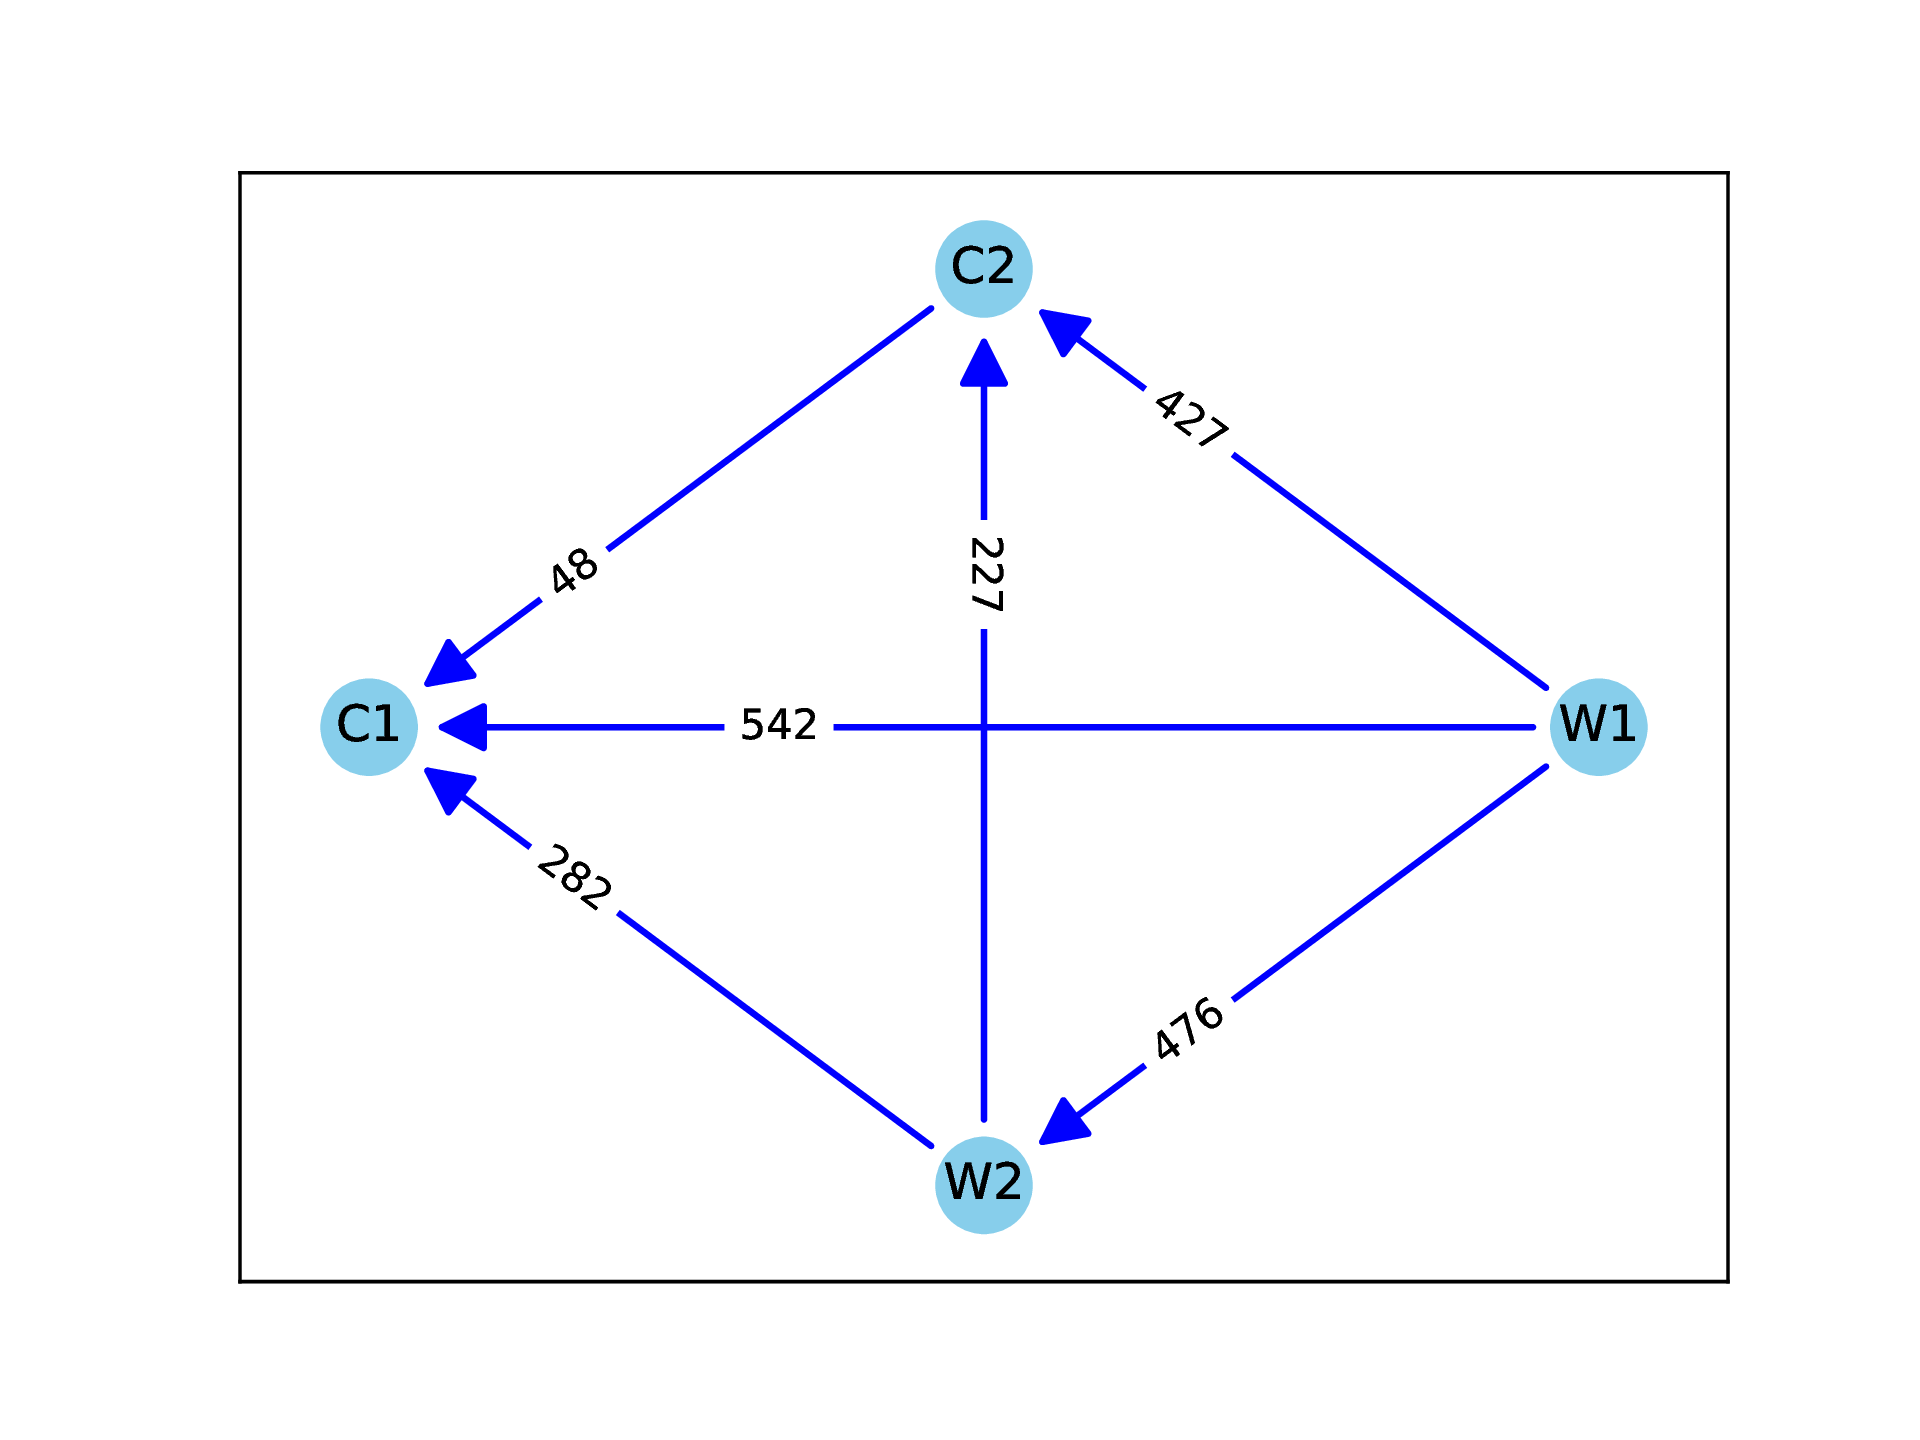
\includegraphics[height=2.5in]{../figures/pwc_graph.png}};
\node at (2.5,-8.2) {\bf Pairwise Comparison Graph};

\node at (10,-5.2) {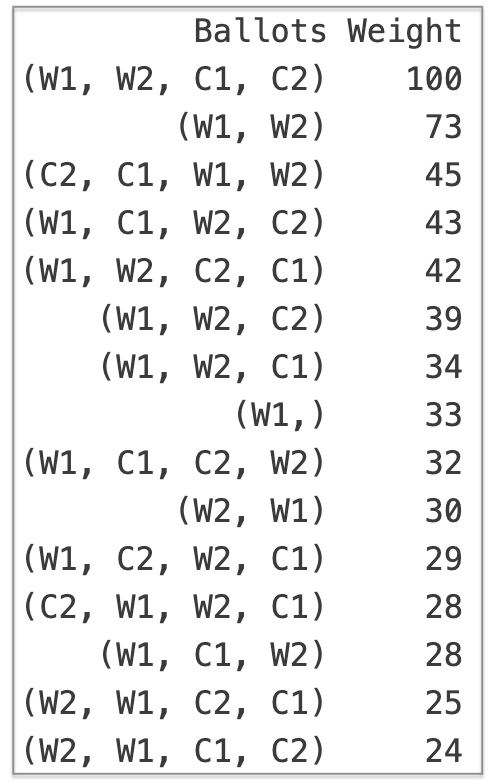
\includegraphics[height=2in]{../figures/profile.png}};
\node at (10,-8.2) {\bf Preference Profile};


\node at (0,0) {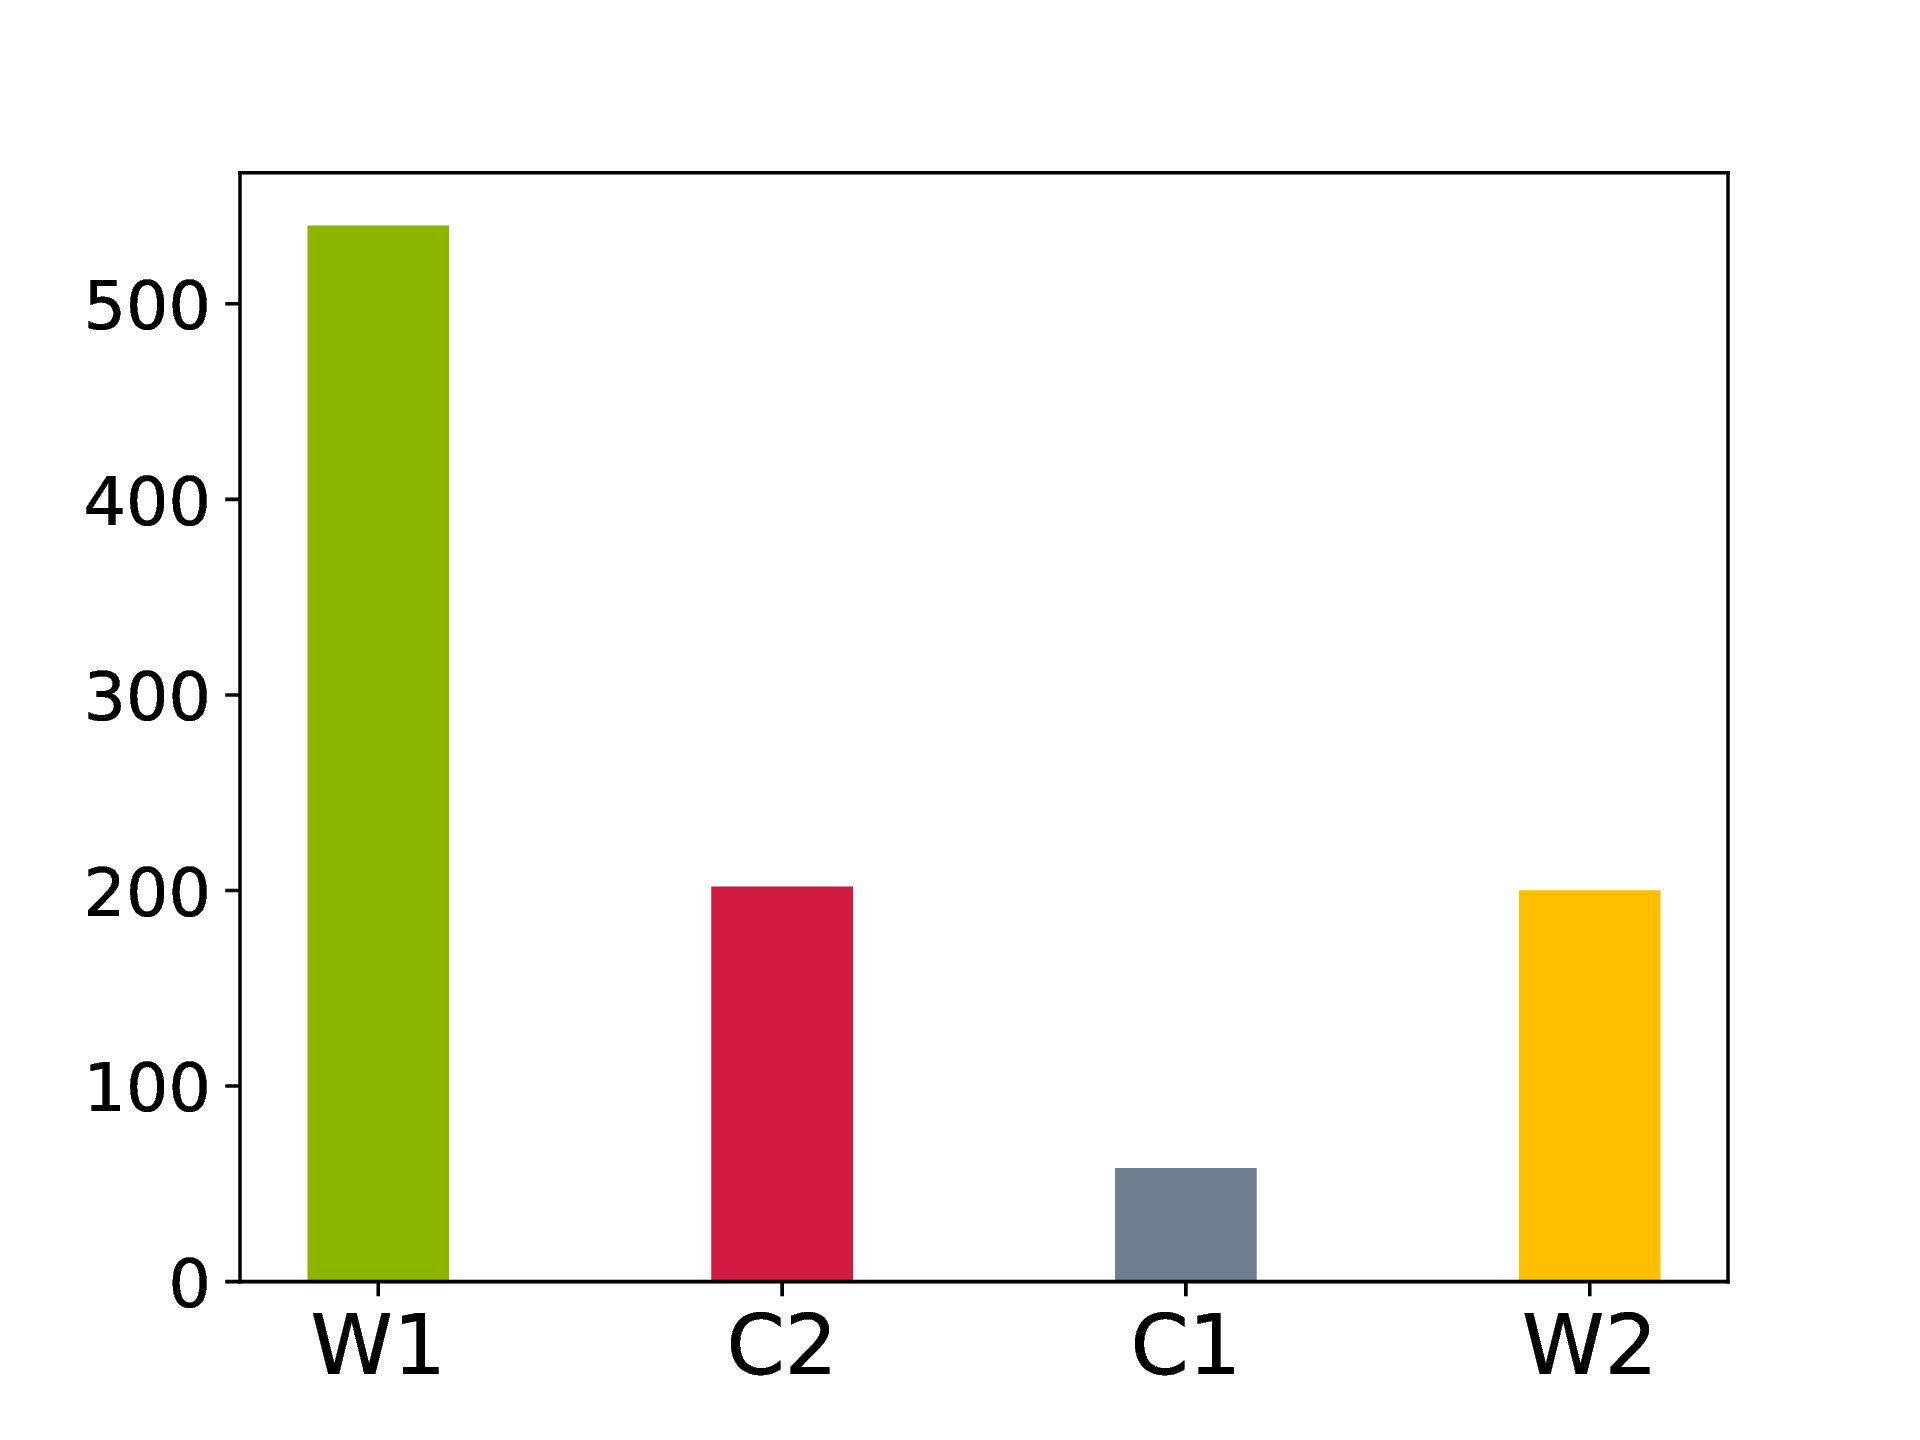
\includegraphics[width=2.5in]{../figures/fpv.png}};
\node at (0,2.2) {\bf First-Place Votes};
\node at (6,0) {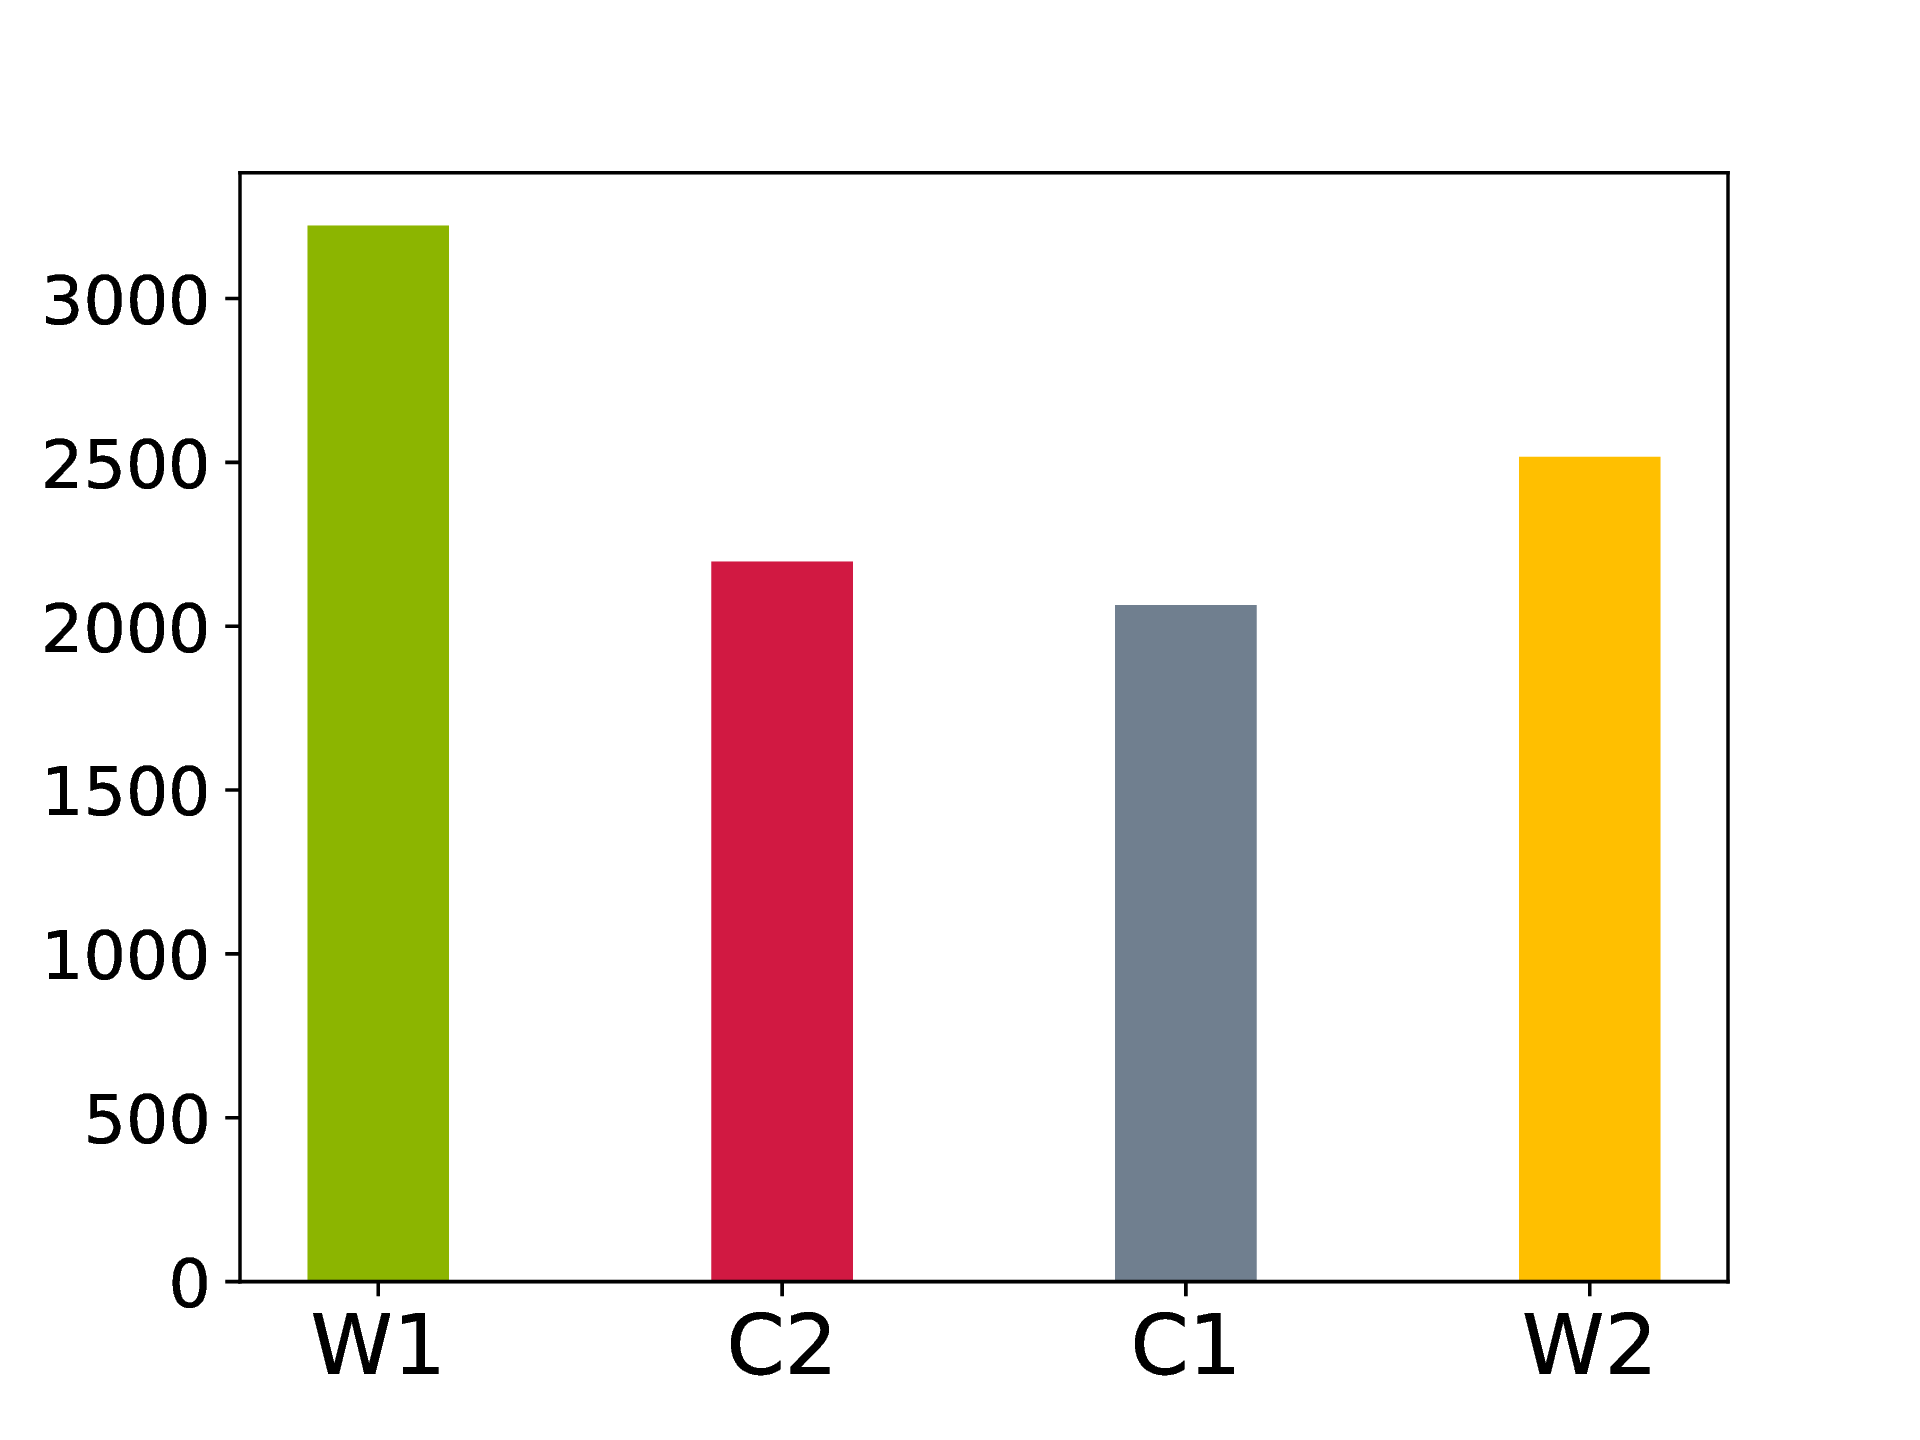
\includegraphics[width=2.5in]{../figures/borda.png}};
\node at (6,2.2) {\bf Borda Points};
\node at (12,0) {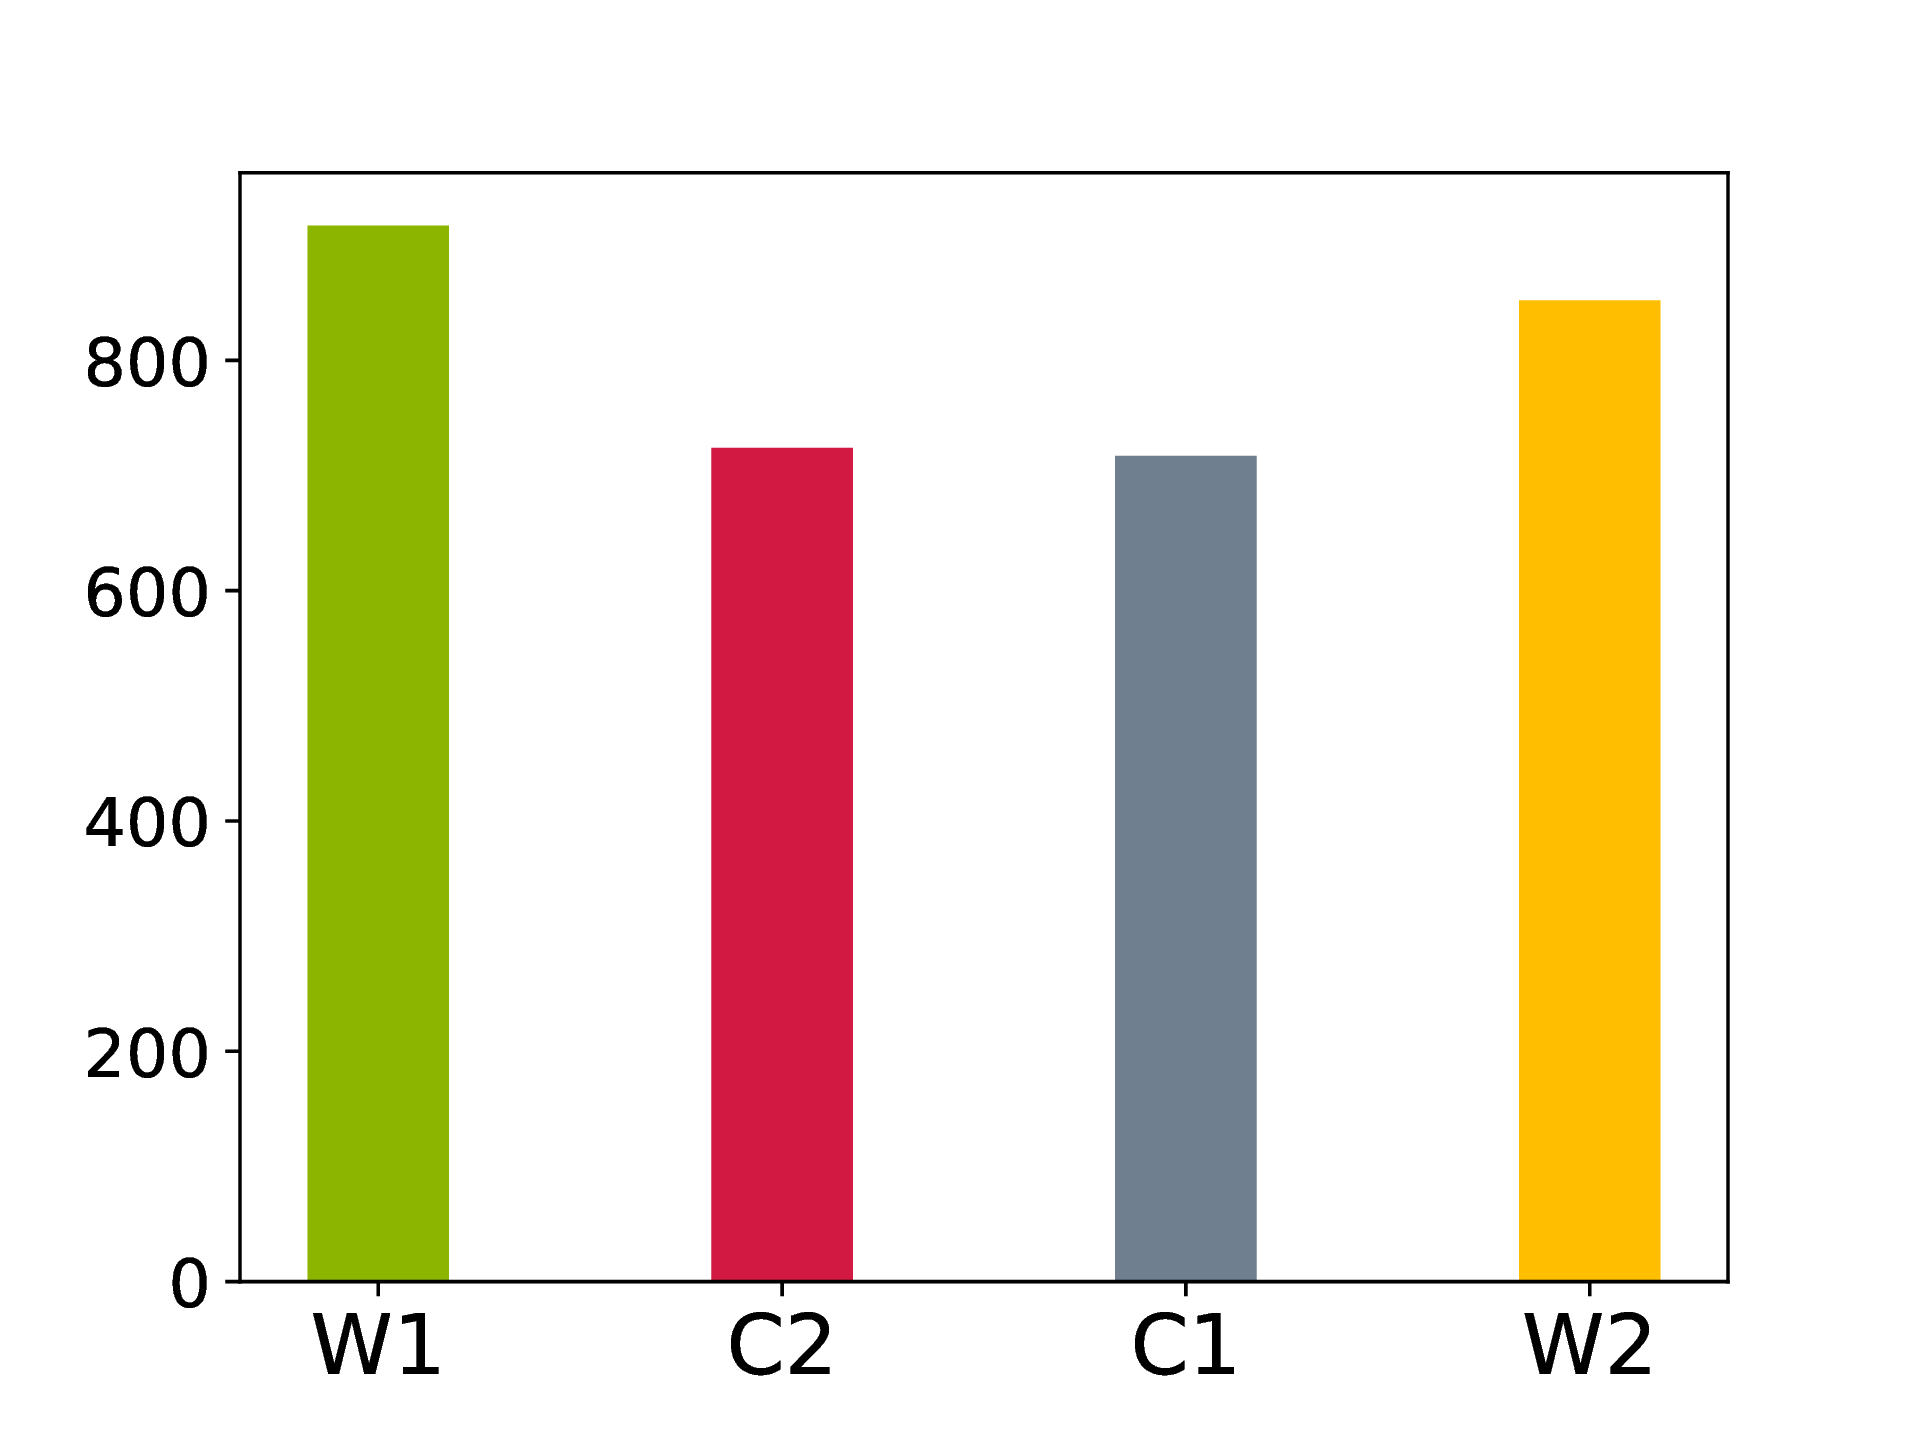
\includegraphics[width=2.5in]{../figures/mentions.png}};
\node at (12,2.2) {\bf Mentions};

\end{tikzpicture}

 \caption{Four visualizations for the same synthetic four-candidate preference profile with 1000 voters.  The profile was generated with the CS model, which produces incomplete ballots at a realistic rate.}
 \label{fig: votekit summary stats}
\end{figure}




For a given preference profile, basic \VK functions provide statistics and visuals for first-place votes, Borda count, and mention frequency, as well as head-to-head comparisons (see Figure \ref{fig: votekit summary stats}).   The pairwise comparison graph shows  head-to-head margins between candidates.  For instance, 282 more voters ranked $W_2>C_1$ than $C_1>W_2$ in the preference profile used to make the figure.  Note that $W_1$, who has the most first-place votes by far, is also preferred head-to-head over all alternatives, making them the {\em Condorcet candidate} in this election.

\FloatBarrier
%%%%%%%%%%%%%%%
\subsection{Area of need: Resources for research}

Previous research works such as \cite{elkind2017multiwinner} have compared properties of earlier generative models; \VK facilitates robust comparisons across a more comprehensive and up-to-date list of alternatives.  It also offers new analytical tools that will support research on elections.
Some examples of more sophisticated functionality are shown in Figure \ref{fig: votekit visualization}.  At left is a {\em ballot graph}, where nodes are ballots weighted by their frequency in the profile; a recent research paper shows that ballot graphs can be metrized to realize classical statistical ranking distances, like Kendall tau and the Spearman footrule \cite{duchin_tapp_24}. 
VoteKit also implements a class of election distances, as surveyed in \cite{distance-elex}.  Choices for measuring the difference between two profiles on the same set of candidates include $L^p$ distance and Wasserstein (earth-mover) distance.  
At right is a multidimensional scaling (MDS) plot of a different set of data, showing mutual $L^1$ differences between generated profiles across various selections of model (shown in colors) and candidate strength parameters (shown with symbols), enabling comparisons in the style of \cite{drawing-a-map}.  


\begin{figure}[bht!]
\begin{tikzpicture}
\node at (0,0) {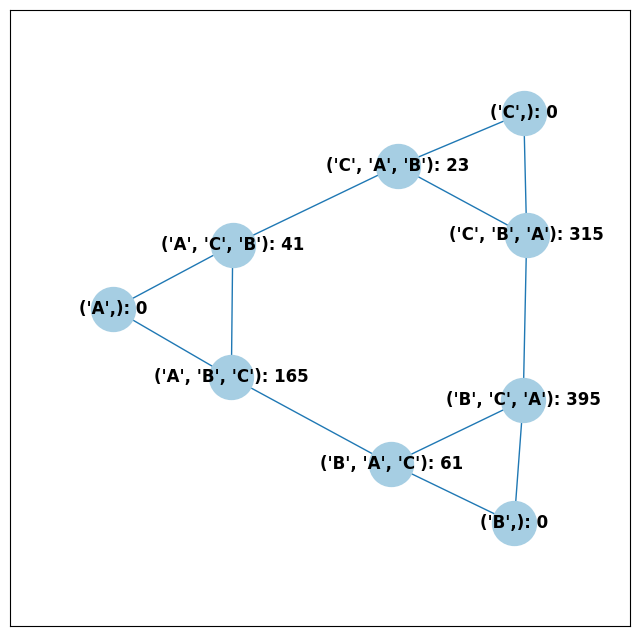
\includegraphics[width=2.5in]{../figures/bg_viz.png}};
\node at (0,3.5) {\bf Ballot Graph};
\node at (8,0) {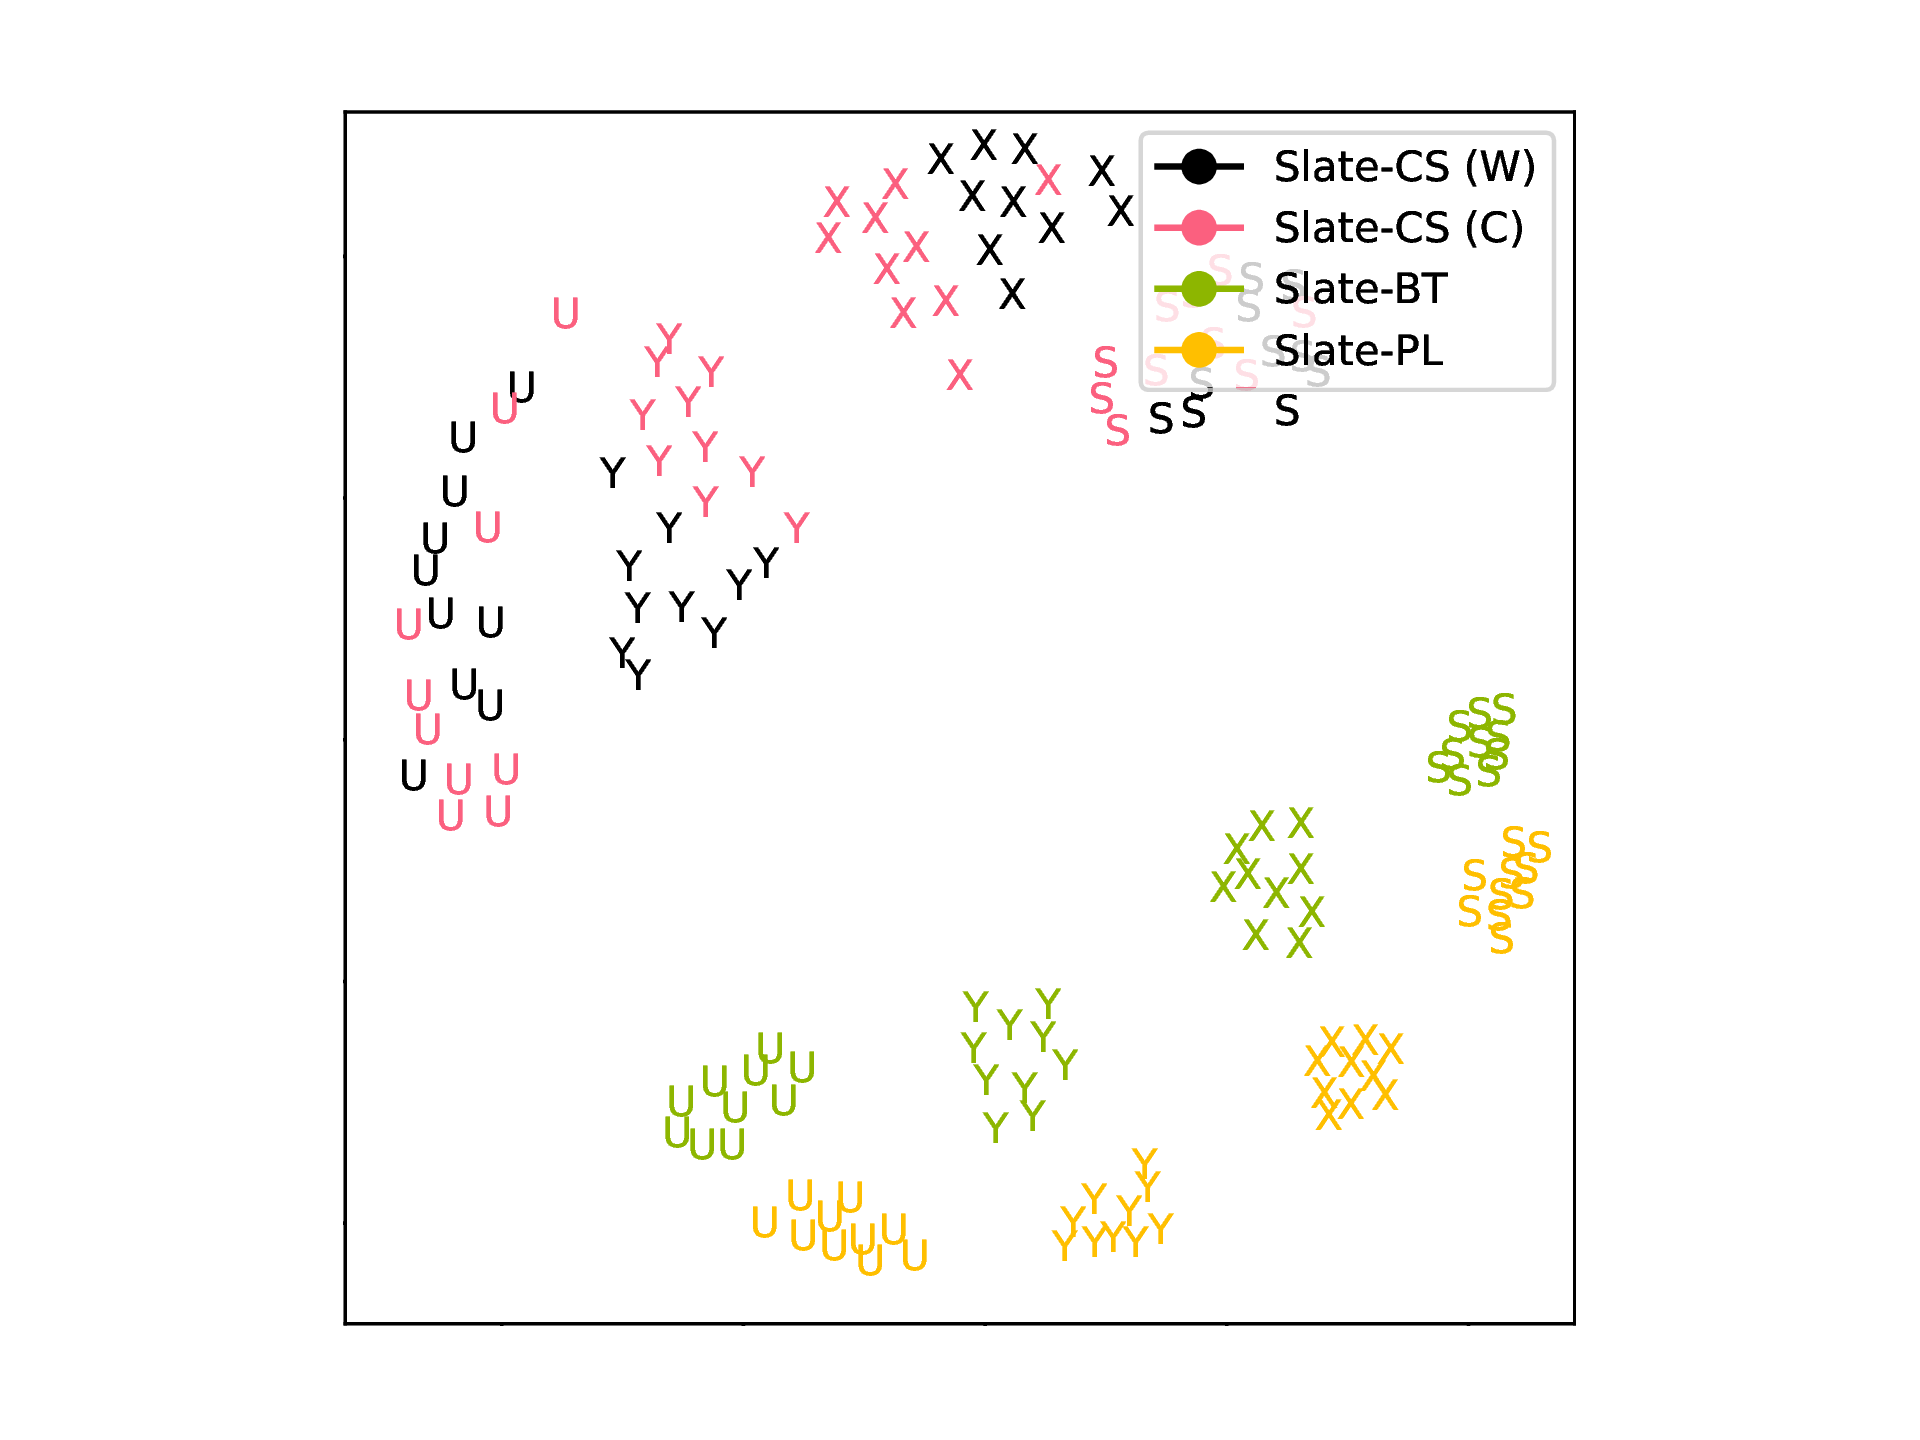
\includegraphics[width=2.4in]{../figures/mds_plot_p_0.7_distance_L_1_seed_47.png}};
\node at (8,3.5) {\bf MDS Plot};
 \end{tikzpicture}
 \caption{At left, the ballot graph for a 3-candidate election.  There is one node per possible ballot, and the weights show the number of instances of that ballot in the profile.  At right, a multidimensional scaling (MDS) plot for 160 synthetic profiles made with various generative models and candidate strength parameters for two slates of 3 candidates each.  
The MDS plot is a low-distortion planar embedding of those 160 profiles and their pairwise differences.}
 \label{fig: votekit visualization}
\end{figure}

Finally, \VK interacts seamlessly with a wide range of actual vote data, such as thousands of political elections collected by FairVote and a cleaned repository of over 1000 Scottish STV local government elections \cite{RCV-Cruncher,Scot-Elex}.  Previously, the use of real data in election research was often extremely limited; for instance, a recent survey reports that the single most popular ``real-life" dataset has been a survey of 5000 respondents' sushi preferences \cite{GuideExperiments}.


\clearpage
%%%
\section{Projects}
A significant number of white papers and scholarly articles have used \VK (and its predecessor codebase) in recent years.
These include the following.
\begin{itemize}
    \item A large number of case studies in ranked-choice modeling, such as studies for the city councils of Chicago, IL \cite{chicago_city} and  Lowell, MA \cite{lowell_city}; the state legislatures of Oregon and Washington \cite{oregon_state,washington_leg}, and a range of county commissions and school boards across the Pacific Northwest \cite{tukwila_school,chelan_county};
    \item A study modeling the impact of proposed legislation called the Fair Representation Act, which would convert U.S. Congressional elections to the single transferable vote system \cite{FairVote};
    \item A detailed study isolating the impacts of varying hypotheses about voter behavior and candidate availability on the Massachusetts legislature \cite{massachusetts_leg};
    \item A peer-reviewed article for an election law audience on the impact of STV elections on minority representation \cite{Benade2021};
    \item A peer-reviewed article for a CS/econ audience that probes whether STV delivers proportional representation \cite{benade_donnay_duchin_weighill_24}; and
    \item A peer-reviewed article for an CS/operations research audience on optimizing to ``learn" blocs and slates in real-world elections \cite{duchin_tapp_24}.
\end{itemize}

\FloatBarrier
%%%%%%%%%%%%%%%

\subsection*{Acknowledgements}
This work was initiated in a research cluster in Summer 2023, funded by the Democracy Fund and graciously hosted at the Faculty of Computing and Data Sciences at Boston University and the Tisch College of Civic Life at Tufts University.  Major contributors to the initiation of the project include 
Brenda Macias, Emarie De La Nuez, Greg Kehne, Jordan Phan, Rory Erlich, 
James Turk, and  David McCune.  Earlier code contributions were made by Chanel Richardson, Anthony Pizzimenti, Gabe Schoenbach, Dylan Phelan, Thomas Weighill, Dara Gold, and Amy Becker.
The authors also thank 
Deb Otis, Peter Rock, Jeanne Clelland, and Michael Parsons for helpful feedback.  FairVote's data repository in Dataverse (\url{https://dataverse.harvard.edu/dataverse/rcv_cvrs}) and {\sf RCV Cruncher} code on GitHub (\url{https://github.com/fairvotereform/rcv_cruncher/}) are excellent open-source efforts that were inspirational for the current project.

\clearpage
\printbibliography
%A list of key references, including to other software addressing related needs. Note that the references should include full names of venues, e.g., journals and conferences, not abbreviations only understood in the context of a specific discipline.
\end{document}
